% Created by tikzDevice version 0.10.1 on 2016-12-16 09:50:11
% !TEX encoding = UTF-8 Unicode
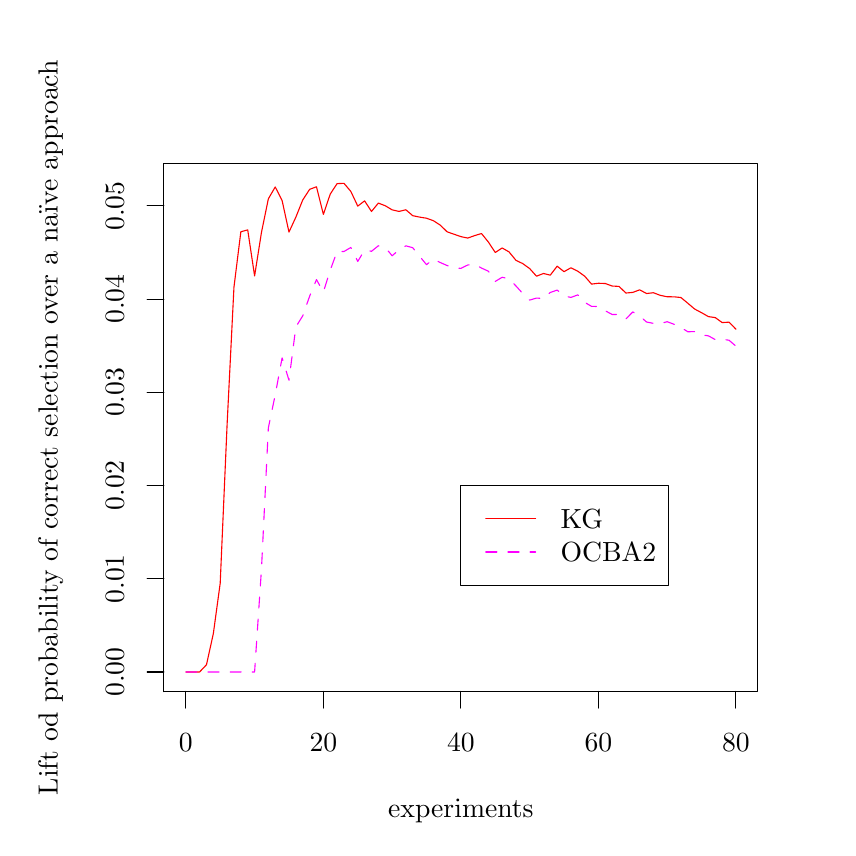
\begin{tikzpicture}[x=1pt,y=1pt]
\definecolor{fillColor}{RGB}{255,255,255}
\path[use as bounding box,fill=fillColor,fill opacity=0.00] (0,0) rectangle (289.08,289.08);
\begin{scope}
\path[clip] ( 49.20, 49.20) rectangle (263.88,239.88);
\definecolor{drawColor}{RGB}{255,0,0}

\path[draw=drawColor,line width= 0.4pt,line join=round,line cap=round] ( 57.15, 56.26) --
	( 59.64, 56.26) --
	( 62.12, 56.26) --
	( 64.61, 58.88) --
	( 67.09, 70.13) --
	( 69.57, 88.33) --
	( 72.06,145.63) --
	( 74.54,195.31) --
	( 77.03,215.33) --
	( 79.51,216.01) --
	( 82.00,199.36) --
	( 84.48,215.10) --
	( 86.97,227.24) --
	( 89.45,231.52) --
	( 91.94,226.60) --
	( 94.42,215.21) --
	( 96.91,220.61) --
	( 99.39,226.81) --
	(101.88,230.65) --
	(104.36,231.59) --
	(106.85,221.59) --
	(109.33,228.95) --
	(111.81,232.73) --
	(114.30,232.82) --
	(116.78,229.90) --
	(119.27,224.60) --
	(121.75,226.49) --
	(124.24,222.66) --
	(126.72,225.69) --
	(129.21,224.73) --
	(131.69,223.25) --
	(134.18,222.68) --
	(136.66,223.27) --
	(139.15,221.13) --
	(141.63,220.63) --
	(144.12,220.22) --
	(146.60,219.33) --
	(149.09,217.72) --
	(151.57,215.30) --
	(154.06,214.44) --
	(156.54,213.57) --
	(159.02,213.05) --
	(161.51,213.94) --
	(163.99,214.69) --
	(166.48,211.61) --
	(168.96,207.83) --
	(171.45,209.47) --
	(173.93,208.06) --
	(176.42,205.03) --
	(178.90,203.82) --
	(181.39,202.03) --
	(183.87,199.27) --
	(186.36,200.25) --
	(188.84,199.66) --
	(191.33,202.89) --
	(193.81,200.91) --
	(196.30,202.32) --
	(198.78,201.07) --
	(201.26,199.29) --
	(203.75,196.42) --
	(206.23,196.72) --
	(208.72,196.63) --
	(211.20,195.72) --
	(213.69,195.58) --
	(216.17,193.19) --
	(218.66,193.42) --
	(221.14,194.35) --
	(223.63,193.01) --
	(226.11,193.30) --
	(228.60,192.35) --
	(231.08,191.84) --
	(233.57,191.82) --
	(236.05,191.57) --
	(238.54,189.50) --
	(241.02,187.40) --
	(243.51,186.08) --
	(245.99,184.67) --
	(248.47,184.31) --
	(250.96,182.51) --
	(253.44,182.67) --
	(255.93,180.12);
\end{scope}
\begin{scope}
\path[clip] (  0.00,  0.00) rectangle (289.08,289.08);
\definecolor{drawColor}{RGB}{0,0,0}

\path[draw=drawColor,line width= 0.4pt,line join=round,line cap=round] ( 57.15, 49.20) -- (255.93, 49.20);

\path[draw=drawColor,line width= 0.4pt,line join=round,line cap=round] ( 57.15, 49.20) -- ( 57.15, 43.20);

\path[draw=drawColor,line width= 0.4pt,line join=round,line cap=round] (106.85, 49.20) -- (106.85, 43.20);

\path[draw=drawColor,line width= 0.4pt,line join=round,line cap=round] (156.54, 49.20) -- (156.54, 43.20);

\path[draw=drawColor,line width= 0.4pt,line join=round,line cap=round] (206.23, 49.20) -- (206.23, 43.20);

\path[draw=drawColor,line width= 0.4pt,line join=round,line cap=round] (255.93, 49.20) -- (255.93, 43.20);

\node[text=drawColor,anchor=base,inner sep=0pt, outer sep=0pt, scale=  1.00] at ( 57.15, 27.60) {0};

\node[text=drawColor,anchor=base,inner sep=0pt, outer sep=0pt, scale=  1.00] at (106.85, 27.60) {20};

\node[text=drawColor,anchor=base,inner sep=0pt, outer sep=0pt, scale=  1.00] at (156.54, 27.60) {40};

\node[text=drawColor,anchor=base,inner sep=0pt, outer sep=0pt, scale=  1.00] at (206.23, 27.60) {60};

\node[text=drawColor,anchor=base,inner sep=0pt, outer sep=0pt, scale=  1.00] at (255.93, 27.60) {80};

\path[draw=drawColor,line width= 0.4pt,line join=round,line cap=round] ( 49.20, 56.26) -- ( 49.20,224.66);

\path[draw=drawColor,line width= 0.4pt,line join=round,line cap=round] ( 49.20, 56.26) -- ( 43.20, 56.26);

\path[draw=drawColor,line width= 0.4pt,line join=round,line cap=round] ( 49.20, 89.94) -- ( 43.20, 89.94);

\path[draw=drawColor,line width= 0.4pt,line join=round,line cap=round] ( 49.20,123.62) -- ( 43.20,123.62);

\path[draw=drawColor,line width= 0.4pt,line join=round,line cap=round] ( 49.20,157.30) -- ( 43.20,157.30);

\path[draw=drawColor,line width= 0.4pt,line join=round,line cap=round] ( 49.20,190.98) -- ( 43.20,190.98);

\path[draw=drawColor,line width= 0.4pt,line join=round,line cap=round] ( 49.20,224.66) -- ( 43.20,224.66);

\node[text=drawColor,rotate= 90.00,anchor=base,inner sep=0pt, outer sep=0pt, scale=  1.00] at ( 34.80, 56.26) {0.00};

\node[text=drawColor,rotate= 90.00,anchor=base,inner sep=0pt, outer sep=0pt, scale=  1.00] at ( 34.80, 89.94) {0.01};

\node[text=drawColor,rotate= 90.00,anchor=base,inner sep=0pt, outer sep=0pt, scale=  1.00] at ( 34.80,123.62) {0.02};

\node[text=drawColor,rotate= 90.00,anchor=base,inner sep=0pt, outer sep=0pt, scale=  1.00] at ( 34.80,157.30) {0.03};

\node[text=drawColor,rotate= 90.00,anchor=base,inner sep=0pt, outer sep=0pt, scale=  1.00] at ( 34.80,190.98) {0.04};

\node[text=drawColor,rotate= 90.00,anchor=base,inner sep=0pt, outer sep=0pt, scale=  1.00] at ( 34.80,224.66) {0.05};

\path[draw=drawColor,line width= 0.4pt,line join=round,line cap=round] ( 49.20, 49.20) --
	(263.88, 49.20) --
	(263.88,239.88) --
	( 49.20,239.88) --
	( 49.20, 49.20);
\end{scope}
\begin{scope}
\path[clip] (  0.00,  0.00) rectangle (289.08,289.08);
\definecolor{drawColor}{RGB}{0,0,0}

\node[text=drawColor,anchor=base,inner sep=0pt, outer sep=0pt, scale=  1.00] at (156.54,  3.60) {experiments};

\node[text=drawColor,rotate= 90.00,anchor=base,inner sep=0pt, outer sep=0pt, scale=  1.00] at ( 10.80,144.54) {Lift od probability of correct selection over a na\"ive approach};
\end{scope}
\begin{scope}
\path[clip] ( 49.20, 49.20) rectangle (263.88,239.88);
\definecolor{drawColor}{RGB}{255,0,255}

\path[draw=drawColor,line width= 0.4pt,dash pattern=on 4pt off 4pt ,line join=round,line cap=round] ( 57.15, 56.26) --
	( 59.64, 56.26) --
	( 62.12, 56.26) --
	( 64.61, 56.26) --
	( 67.09, 56.26) --
	( 69.57, 56.26) --
	( 72.06, 56.26) --
	( 74.54, 56.26) --
	( 77.03, 56.26) --
	( 79.51, 56.26) --
	( 82.00, 56.26) --
	( 84.48, 93.43) --
	( 86.97,144.47) --
	( 89.45,156.41) --
	( 91.94,169.78) --
	( 94.42,161.69) --
	( 96.91,180.96) --
	( 99.39,184.94) --
	(101.88,192.03) --
	(104.36,198.04) --
	(106.85,193.55) --
	(109.33,201.46) --
	(111.81,208.22) --
	(114.30,208.20) --
	(116.78,209.66) --
	(119.27,204.60) --
	(121.75,208.74) --
	(124.24,208.27) --
	(126.72,210.27) --
	(129.21,209.70) --
	(131.69,206.65) --
	(134.18,208.81) --
	(136.66,210.25) --
	(139.15,209.56) --
	(141.63,206.47) --
	(144.12,203.44) --
	(146.60,205.49) --
	(149.09,204.21) --
	(151.57,203.12) --
	(154.06,202.32) --
	(156.54,202.09) --
	(159.02,203.32) --
	(161.51,203.62) --
	(163.99,202.21) --
	(166.48,201.07) --
	(168.96,197.38) --
	(171.45,198.88) --
	(173.93,198.36) --
	(176.42,195.76) --
	(178.90,193.03) --
	(181.39,190.64) --
	(183.87,191.37) --
	(186.36,191.21) --
	(188.84,193.39) --
	(191.33,194.26) --
	(193.81,192.19) --
	(196.30,191.59) --
	(198.78,192.53) --
	(201.26,189.84) --
	(203.75,188.38) --
	(206.23,188.31) --
	(208.72,186.77) --
	(211.20,185.44) --
	(213.69,185.44) --
	(216.17,183.83) --
	(218.66,186.36) --
	(221.14,184.90) --
	(223.63,182.71) --
	(226.11,182.23) --
	(228.60,182.14) --
	(231.08,182.83) --
	(233.57,181.89) --
	(236.05,180.75) --
	(238.54,179.20) --
	(241.02,179.25) --
	(243.51,178.09) --
	(245.99,177.72) --
	(248.47,176.36) --
	(250.96,176.49) --
	(253.44,176.13) --
	(255.93,173.99);
\definecolor{drawColor}{RGB}{0,0,0}

\path[draw=drawColor,line width= 0.4pt,line join=round,line cap=round] (156.54,123.62) rectangle (231.61, 87.62);
\definecolor{drawColor}{RGB}{255,0,0}

\path[draw=drawColor,line width= 0.4pt,line join=round,line cap=round] (165.54,111.62) -- (183.54,111.62);
\definecolor{drawColor}{RGB}{255,0,255}

\path[draw=drawColor,line width= 0.4pt,dash pattern=on 4pt off 4pt ,line join=round,line cap=round] (165.54, 99.62) -- (183.54, 99.62);
\definecolor{drawColor}{RGB}{0,0,0}

\node[text=drawColor,anchor=base west,inner sep=0pt, outer sep=0pt, scale=  1.00] at (192.54,108.18) {KG};

\node[text=drawColor,anchor=base west,inner sep=0pt, outer sep=0pt, scale=  1.00] at (192.54, 96.18) {OCBA2};
\end{scope}
\end{tikzpicture}
